\chapter{Experimental Results}
\label{chap:experimental-results}

In this chapter, we evaluate and compare the synthesizers presented in
Chapter~\ref{chap:synthesis}.
The synthesizers are compared in terms of their running time and number of
solved problems.
A description of the benchmarks is provided in Section~\ref{sec:bench-desc}.
Section~\ref{sec:results} presents the results of the benchmarks
and a comparison between the setwise synthesizer
(Section~\ref{sec:setwise-encoding}) and the whole synthesizer
(Section~\ref{sec:whole-encoding}).

\section{Benchmark Description}
\label{sec:bench-desc}

A set of 285522 expressions were provided by OutSystems.
We conducted an analysis to determine which builtin functions and which
combinations were the most common in that set.
We picked 51 expressions containing only those functions (see
Table~\ref{table:builtin-description}) with sizes (number of components) ranging
from 1 to 7.
A description of these 51 expressions in terms of size is shown in
Figure~\ref{fig:bar-chart-sizes-51}.

\begin{figure}
  \centering
  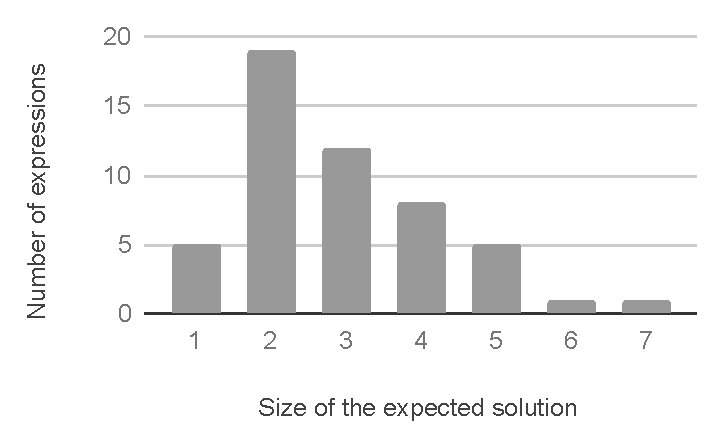
\includegraphics[width=0.5\textwidth]{assets/bar-chart-sizes-51.pdf}
  \caption{Number of expressions per size. For example, there are 31
    expressions of size 2, and 16 expressions of size 1, out of 51 expressions.}
  \label{fig:bar-chart-sizes-51}
\end{figure}

The hardness of a benchmark depends on the size of the solution, the number of
input-output examples, and the library of components.
Typically, the higher the size and the number of components, the harder it is to
synthesize a program.
% Moreover, a library containing components which must be encoded to recursive
% formulas (\lstinline{Replace}, \lstinline{ToLower}, \lstinline{ToUpper},
% \lstinline{Trim}, \lstinline{TrimStart}, and \lstinline{TrimEnd}) makes the
% synthesis problem much harder than if we just had a library whose components
% had a direct counterpart in some \gls{smt} theory.
Figure~\ref{fig:bar-chart-components-freq-51} shows in how many expressions each
component occurs.

\begin{figure}
  \centering
  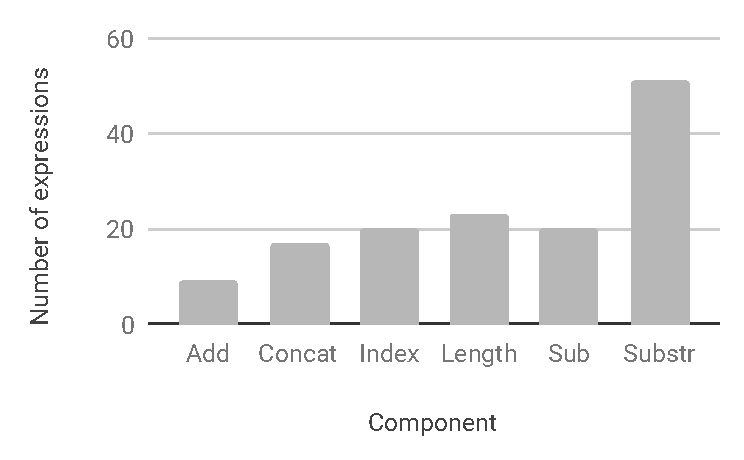
\includegraphics[width=0.5\textwidth]{assets/bar-chart-components-freq-51.pdf}
  \caption{Number of expressions per component.}
  \label{fig:bar-chart-components-freq-51}
\end{figure}

We obtained a set of 3 input-output examples for each of these 51 expressions.
In order to do that, we developed an \textit{interpreter} for OutSystems
expressions, and manually created a set of 3 different inputs for each
expression.
The inputs were carefully crafted in order to try to eliminate as much ambiguity
as possible.
Then we interpreted the expressions over their set of inputs in order to
obtain the correspondent outputs.
A first approach was tried, where we encoded the expressions in \gls{smt} in
such a way that a solution to the formulas yielded valid input-output examples.
Although the approach ``worked'', it was ultimately too slow, and the
automatically generated examples were not natural, so we resorted to the manual
approach.

The \gls{smt} solver used to solve the formulas generated in the synthesis
process was Z3 version 4.8.5~\cite{DeMoura:2008:ZES}.
Each benchmark was monitored by the \textit{runsolver}
program~\cite{Roussel:2011:JSAT}, and restricted to a time limit of 10 minutes
and a memory limit of 16 GB.

\section{Results}
\label{sec:results}

We are interested in the relation between the number and quality of the
input-output examples, and their impact on synthesis time and program quality.
In this section, we only study the impact of the number of input-output
examples.

We present the results for both synthesizers discussed in
Chapter~\ref{chap:synthesis} with the following configurations.
For each instance of 3 input-output examples we ran both synthesizers using 1,
2, or all 3 of the input-output examples.
We ran the Setwise synthesizer (Section~\ref{sec:setwise-encoding}) configured
to synthesize programs with a maximum of one integer and one string constants
(configurations S-e1:c1, S-e2:c1, and S-e3:c1, for 1, 2, and 3 input-output
examples, respectively).
We ran the Whole synthesizer (Section~\ref{sec:whole-encoding}) configured to
synthesize programs with a maximum of one constant, which the synthesizer can
choose whether it is a an integer or a string (configurations W-e1:c1, W-e2:c1,
and W-e3:c1, for for 1, 2, and 3 input-output examples, respectively).

Figures~\ref{fig:bar-chart-solved-S-e1-c1}, \ref{fig:bar-chart-solved-S-e2-c1},
and \ref{fig:bar-chart-solved-S-e3-c1} show the number of solved instances per
size of the expected solution for S-e1:c1, S-e2:c1, and S-e3:c1, respectively,
where by solved we mean that the synthesizer outputs a program that satisfies
the input-output examples.
Figures~\ref{fig:bar-chart-solved-W-e1-c1}, \ref{fig:bar-chart-solved-W-e2-c1},
and \ref{fig:bar-chart-solved-W-e3-c1} show the same for W-e1:c1, W-e2:c1, and
W-e3:c1, respectively.

Figures~\ref{fig:bar-chart-expected-S-e1-c1}, \ref{fig:bar-chart-expected-S-e2-c1},
and \ref{fig:bar-chart-expected-S-e3-c1} show the number of solved instances per
size of the expected solution for S-e1:c1, S-e2:c1, and S-e3:c1, respectively,
where by solved we mean that the synthesizer outputs a program that, not only
satisfies the input-output examples, but also matches the expected solution.
Matching the expected solution does not necessarily mean that the program is
exactly equal to the expected solution, but rather that it captures the original
intent and generalizes to more examples.
Figures~\ref{fig:bar-chart-expected-W-e1-c1}, \ref{fig:bar-chart-expected-W-e2-c1},
and \ref{fig:bar-chart-expected-W-e3-c1} show the same for W-e1:c1, W-e2:c1, and
W-e3:c1, respectively.

% Solved Setwise
\begin{figure}
  \centering
  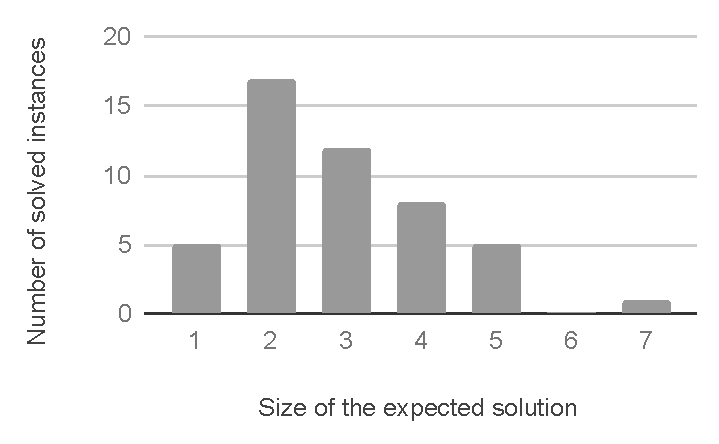
\includegraphics[width=0.5\textwidth]{assets/bar-chart-solved-S-e1-c1.pdf}
  \caption{Number of solved instances per size of the expected solution for
    the Setwise synthesizer with one example, one integer constant, and one
    string constant (S-e1:c1). Here by solved we mean that the synthesizer
    outputs a program that satisfies the input-output examples.}
  \label{fig:bar-chart-solved-S-e1-c1}
\end{figure}

\begin{figure}
  \centering
  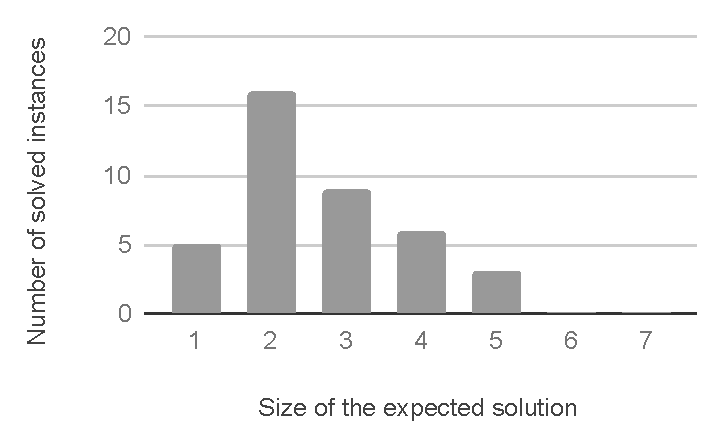
\includegraphics[width=0.5\textwidth]{assets/bar-chart-solved-S-e2-c1.pdf}
  \caption{Number of solved instances per size of the expected solution for
    the Setwise synthesizer with two examples, one integer constant, and one
    string constant (S-e2:c1). Here by solved we mean that the synthesizer
    outputs a program that satisfies the input-output examples.}
  \label{fig:bar-chart-solved-S-e2-c1}
\end{figure}

\begin{figure}
  \centering
  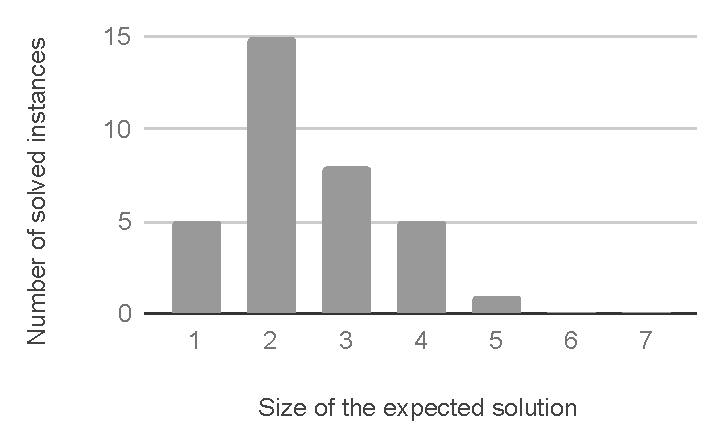
\includegraphics[width=0.5\textwidth]{assets/bar-chart-solved-S-e3-c1.pdf}
  \caption{Number of solved instances per size of the expected solution for
    the Setwise synthesizer with three examples, one integer constant, and one
    string constant (S-e3:c1). Here by solved we mean that the synthesizer
    outputs a program that satisfies the input-output examples.}
  \label{fig:bar-chart-solved-S-e3-c1}
\end{figure}

% Expected Setwise
\begin{figure}
  \centering
  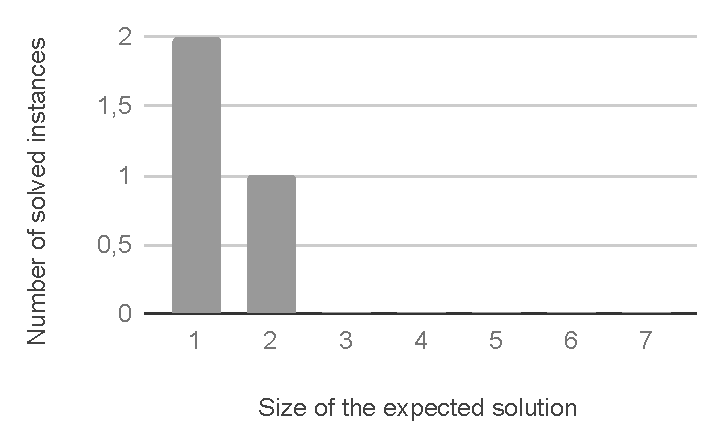
\includegraphics[width=0.5\textwidth]{assets/bar-chart-expected-S-e1-c1.pdf}
  \caption{Number of solved instances per size of the expected solution for
    the Setwise synthesizer with one example, one integer constant, and one
    string constant (S-e1:c1). Here by solved we mean that the synthesizer
    outputs a program that matches the expected solution, and generalizes to
    more examples.}
  \label{fig:bar-chart-expected-S-e1-c1}
\end{figure}

\begin{figure}
  \centering
  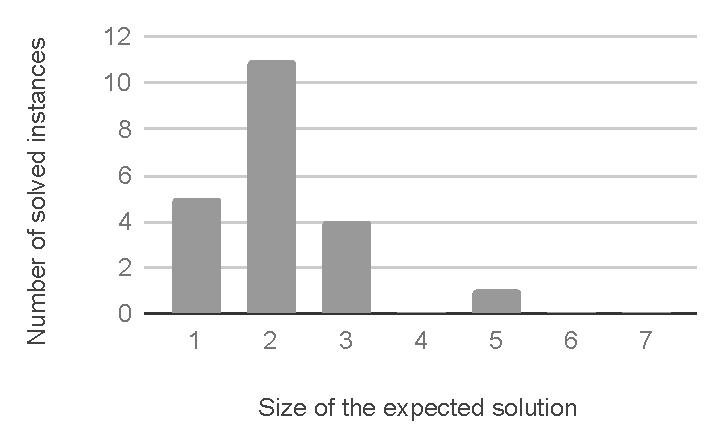
\includegraphics[width=0.5\textwidth]{assets/bar-chart-expected-S-e2-c1.pdf}
  \caption{Number of solved instances per size of the expected solution for
    the Setwise synthesizer with two examples, one integer constant, and one
    string constant (S-e2:c1). Here by solved we mean that the synthesizer
    outputs a program that matches the expected solution, and generalizes to
    more examples.}
  \label{fig:bar-chart-expected-S-e2-c1}
\end{figure}

\begin{figure}
  \centering
  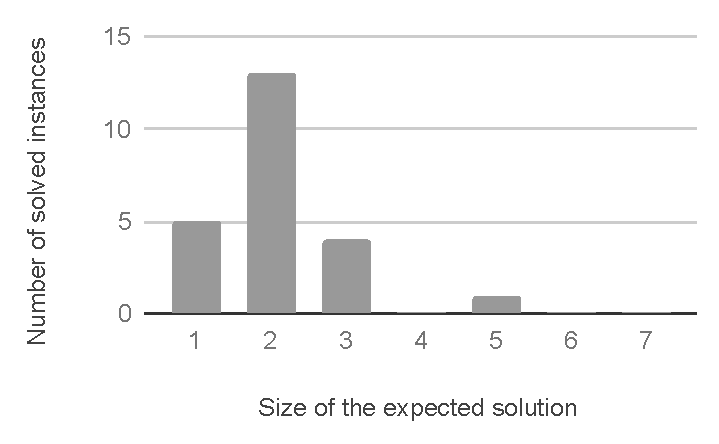
\includegraphics[width=0.5\textwidth]{assets/bar-chart-expected-S-e3-c1.pdf}
  \caption{Number of solved instances per size of the expected solution for
    the Setwise synthesizer with three examples, one integer constant, and one
    string constant (S-e3:c1). Here by solved we mean that the synthesizer
    outputs a program that matches the expected solution, and generalizes to
    more examples.}
  \label{fig:bar-chart-expected-S-e3-c1}
\end{figure}

% Solved Whole
\begin{figure}
  \centering
  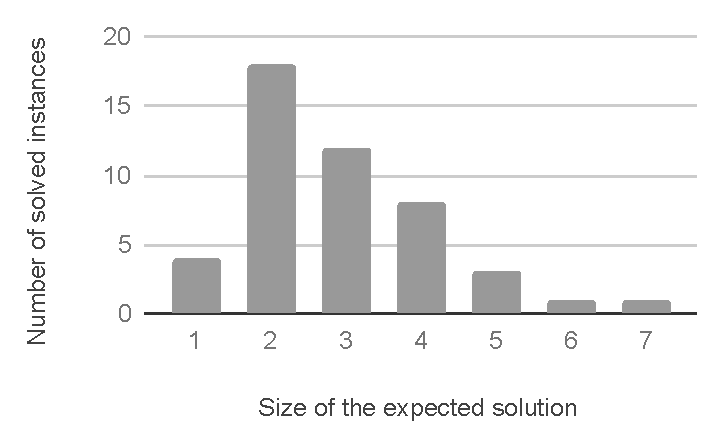
\includegraphics[width=0.5\textwidth]{assets/bar-chart-solved-W-e1-c1.pdf}
  \caption{Number of solved instances per size of the expected solution for
    the Whole synthesizer with one example, one integer constant, and one
    string constant (W-e1:c1). Here by solved we mean that the synthesizer
    outputs a program that satisfies the input-output examples.}
  \label{fig:bar-chart-solved-W-e1-c1}
\end{figure}

\begin{figure}
  \centering
  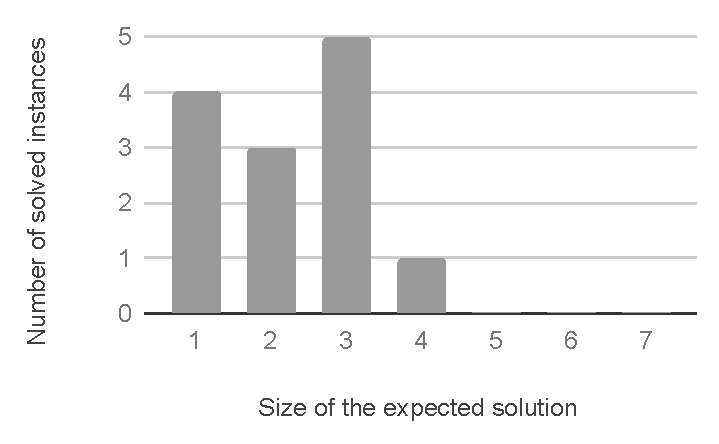
\includegraphics[width=0.5\textwidth]{assets/bar-chart-solved-W-e2-c1.pdf}
  \caption{Number of solved instances per size of the expected solution for
    the Whole synthesizer with two examples, one integer constant, and one
    string constant (W-e2:c1). Here by solved we mean that the synthesizer
    outputs a program that satisfies the input-output examples.}
  \label{fig:bar-chart-solved-W-e2-c1}
\end{figure}

\begin{figure}
  \centering
  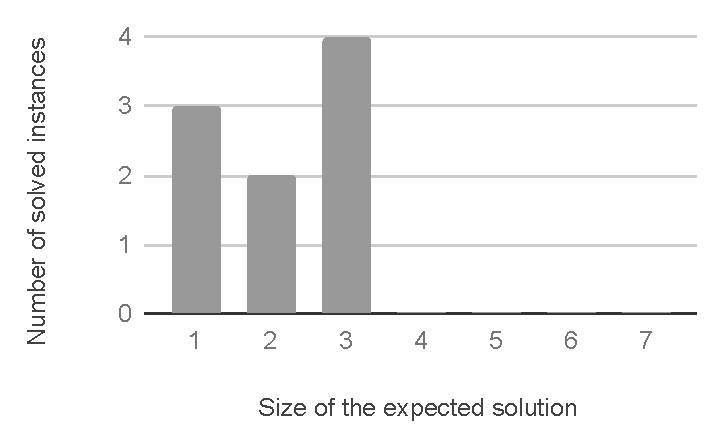
\includegraphics[width=0.5\textwidth]{assets/bar-chart-solved-W-e3-c1.pdf}
  \caption{Number of solved instances per size of the expected solution for
    the Whole synthesizer with three examples, one integer constant, and one
    string constant (W-e3:c1). Here by solved we mean that the synthesizer
    outputs a program that satisfies the input-output examples.}
  \label{fig:bar-chart-solved-W-e3-c1}
\end{figure}

% Expected Whole
\begin{figure}
  \centering
  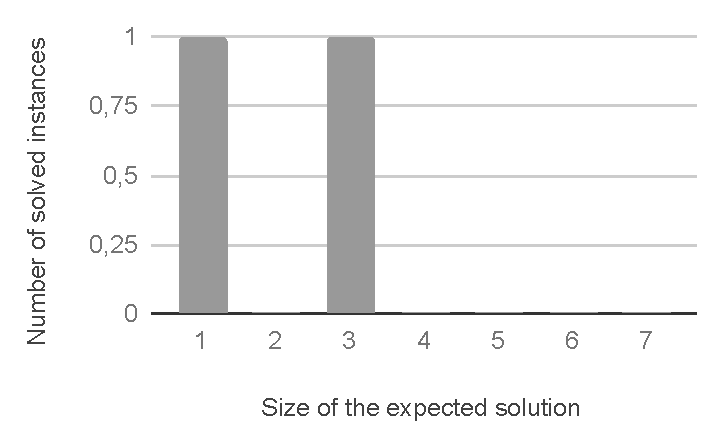
\includegraphics[width=0.5\textwidth]{assets/bar-chart-expected-W-e1-c1.pdf}
  \caption{Number of solved instances per size of the expected solution for
    the Whole synthesizer with one example, one integer constant, and one
    string constant (W-e1:c1). Here by solved we mean that the synthesizer
    outputs a program that matches the expected solution, and generalizes to
    more examples.}
  \label{fig:bar-chart-expected-W-e1-c1}
\end{figure}

\begin{figure}
  \centering
  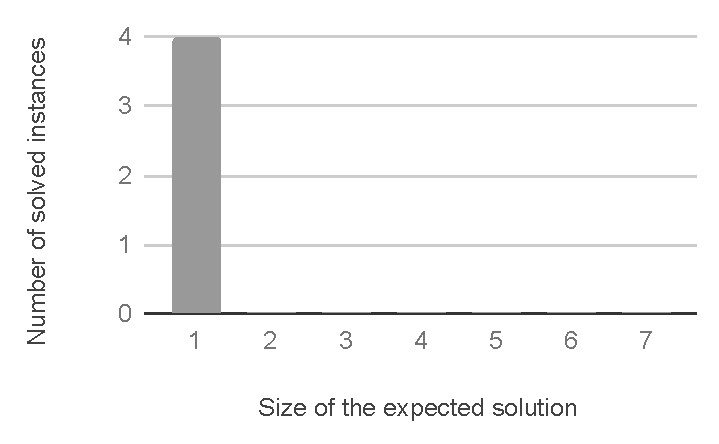
\includegraphics[width=0.5\textwidth]{assets/bar-chart-expected-W-e2-c1.pdf}
  \caption{Number of solved instances per size of the expected solution for
    the Whole synthesizer with two examples, one integer constant, and one
    string constant (W-e2:c1). Here by solved we mean that the synthesizer
    outputs a program that matches the expected solution, and generalizes to
    more examples.}
  \label{fig:bar-chart-expected-W-e2-c1}
\end{figure}

\begin{figure}
  \centering
  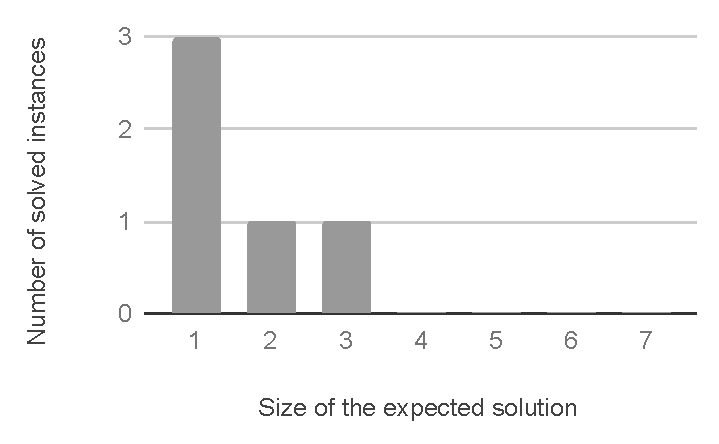
\includegraphics[width=0.5\textwidth]{assets/bar-chart-expected-W-e3-c1.pdf}
  \caption{Number of solved instances per size of the expected solution for
    the Whole synthesizer with three examples, one integer constant, and one
    string constant (W-e3:c1). Here by solved we mean that the synthesizer
    outputs a program that matches the expected solution, and generalizes to
    more examples.}
  \label{fig:bar-chart-expected-W-e3-c1}
\end{figure}

\section{Discussion}
\label{sec:discussion}
